\documentclass[12pt,a4paper]{article}
\usepackage[italian]{babel}
\usepackage[T1]{fontenc}
\usepackage[latin1]{inputenc}
\usepackage{graphicx}
\usepackage{amsmath}
\usepackage{subfig}
\usepackage[a4paper,top=1.5cm,bottom=1.4cm,left=1.4cm,right=1.4cm]{geometry}
\date{}
\begin{document}
\title{Ipersonica\\ Esercitazione 3 \\ Prof.re Renato Paciorri}
\author{Matteo Hakimi 1455230}
\maketitle
\begin{figure}[htbp]
\centering

\includegraphics[width=100mm]{Immagini/1}
\end{figure}
\newpage
\tableofcontents
\newpage
\section{Introduzione}
Si vuole analizzare il fenomeno dell'interazione viscosa per una lastra piana  immersa in una corrente ipersonica, considerando diverse condizioni di volo, e andando a determinare l'estensione della regione di interazione forte che si ha nella lastra piana stessa.
\begin{figure}[htbp]
	\centering
	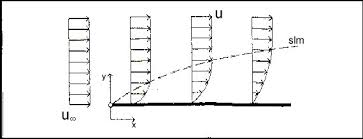
\includegraphics[width=100mm]{Immagini/strato}
	\caption{Lastra piana}
\end{figure}

\section{Interazione viscosa per la lastra piana}
Si consideri una lastra piana isoterma a $T_{w}=600K$ immersa in una corrente ipersonica a $M=12$, nelle seguenti condizioni di volo $T_{\infty}=288K$ e $p_{\infty}=2Pa$. In queste condizioni, il flusso che si viene a creare in prossimit� della lastra stessa, � tale che non � possibile disaccoppiare la soluzione esterna da quella interna intendendo che esiste una mutua interazione tra strato limite e soluzione esterna.
Detto $\delta^*$, lo spessore di spostamento, il parametro di similitudine ipersonica $K$ diventa:\\

$$K=\frac{d\delta^*}{dx}M$$
Si vuole determinare l'estensione della prima regione in cui ricordiamo:\\
$$K=\frac{d\delta^*}{dx}M>1$$
$$\frac{p_{e}}{p_{\infty}}=1+\frac{\gamma(\gamma+1)}{4}K^2+\gamma K^2\sqrt{(\frac{\gamma+1}{4})^2+\frac{1}{K^2}}$$
In base alla definizione di $K$, e dell'ordine di grandezza che assume nelle varie zone di interazione (forte e debole), possiamo pensare di cercare il confine tra queste ultime per un valore di $K$ prossimo a 1.\\
Sappiamo inoltre che nel caso di interazione forte:\\
$$K^2\approx\chi=\frac{M_{\infty}^3}{\sqrt{Re_{x}}}\sqrt{C}$$
dove $C=\frac{\rho_{w}\mu_{w}}{\rho_{e}\mu_{e}}=\frac{T_{\infty}\mu_{w}}{T_{w}\mu_{\infty}}$.\\ Utilizzando la legge di Sutherland per la viscosit� si ottiene ,per queste condizioni di volo, $C\approx0.81$.\\
Imponendo $K=1$, dal numero di Reynolds locale cosi definito $Re_{x}=\frac{\rho_{\infty} u_{\infty} x}{\mu_{\infty}}$, con x contato a partire dal bordo d'attacco, ricavo che la distanza $x_{int}=436.2m$, si osserva come tale dimensione sia di qualche ordine di grandezza maggiore rispetto a quelle che sono le lunghezze caratteristiche dei velivoli, vedremo in seguito come tale lunghezza sia fortemente influenzata dalle condizioni di volo, e come sia estremamente sensibili a piccole variazioni sulle stesse.\\
Per completezza si il valore del rapporto delle pressioni per la stessa lastra nelle stesse condizioni di volo ad una distanza dal bordo d'attacco pari a $L=10m$.\\
Nella zona di interazione forte sappiamo che:\\
$$\frac{p_{e}}{p_{\infty}}\approx 1+a\chi$$
dove $a=0.5$, e $\chi=6.6$  poich� $Re_{x}=54761$, si ha che $\frac{p_{e}}{p_{\infty}}=4.3$ 

\section{Interazione viscosa al variare delle condizioni di volo}
Come detto nella sezione precedente la zona di interazione viscosa forte presenta un'elevata sensibilit� dalle condizioni di volo.\\In questa sezione si vuole analizzare in che modo, questa estensione, varia al variare dei parametri di volo: quota e velocit� ovvero $M$ e $p_{\infty}$. 

\subsection{Intereazione viscosa al variare del Mach}
In questa sezione si vuole analizzare la variazione dell'estensione della zona di interazione viscosa forte per una lastra piana, al variare del numero di Mach, avendo fissato la quota ovvero la pressione all'infinito $p_{\infty}$. Nella fattispecie il calcolo che seguir� verra effettuato avendo scelto $p_{\infty}=10^5Pa$.\\
Si riportano i risultati in forma grafica.
\begin{figure}[htbp!]
	\centering
	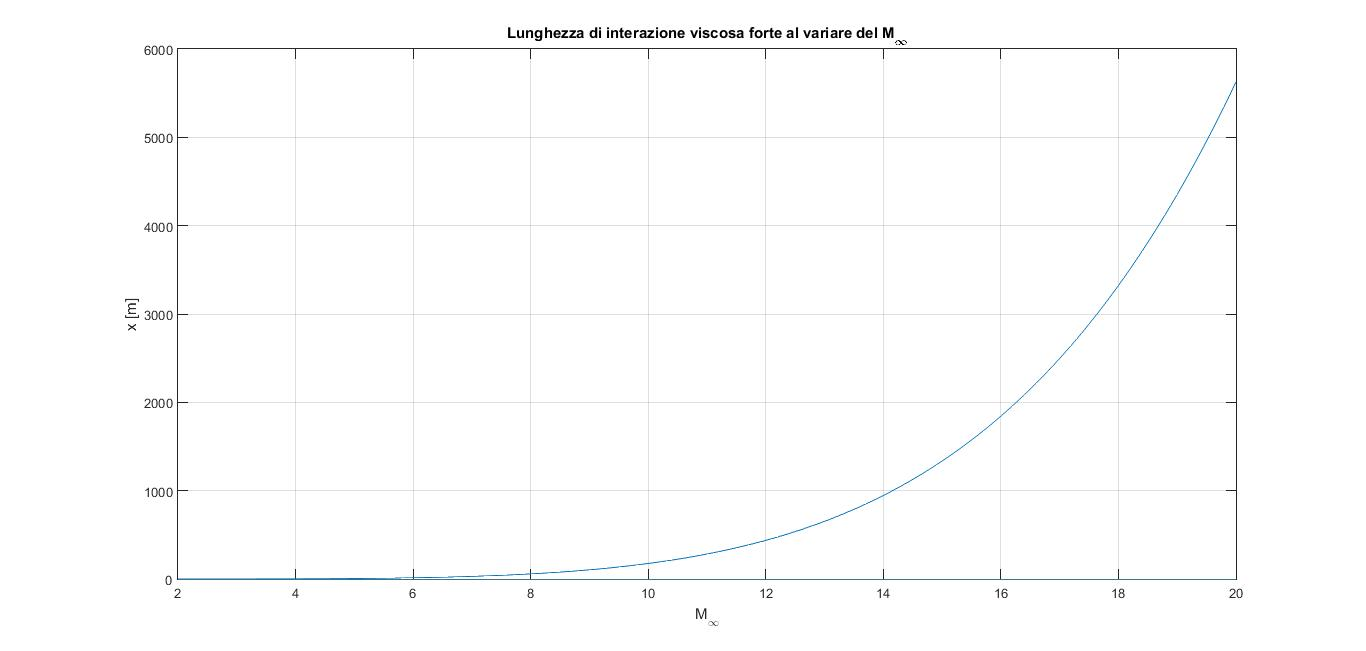
\includegraphics[width=150mm]{Immagini/L_Mach}
	\caption{Estensione della zona di interazione viscosa forte al variare del numero di Mach}
\end{figure}\\
Si nota come all'aumentare del numero di Mach, l'estensione della zona di interazione cresce repentinamente passando da valori dell'ordine del millimetro a valori di centinaia o migliaia di metri.\\
Una spiegazione di tale comportamento risiede nel fatto che all'aumentare del numero di Mach, l'urto generato al bordo d'attacco tende ad accostarsi sempre di pi� alla parete, riducendo il cosiddetto strato d'urto, e rendendo la mutua interazione di natura sempre pi� intensa.\\

\subsection{Interazione viscosa al variare della pressione}
In questa sezione si vuole analizzare la variazione dell'estensione della zona di interazione viscosa forte per una lastra piana, al variare del numero della quota ovvero della pressione all'infinito, avendo fissato il numero di Mach di volo.\\
Nella fattispecie il calcolo che seguir� verra effettuato avendo fissato il Mach di volo ad un valore pari a $M=2$.\\
Si riportano i risultati in forma grafica.
\newpage
\begin{figure}[htbp!]
	\centering
	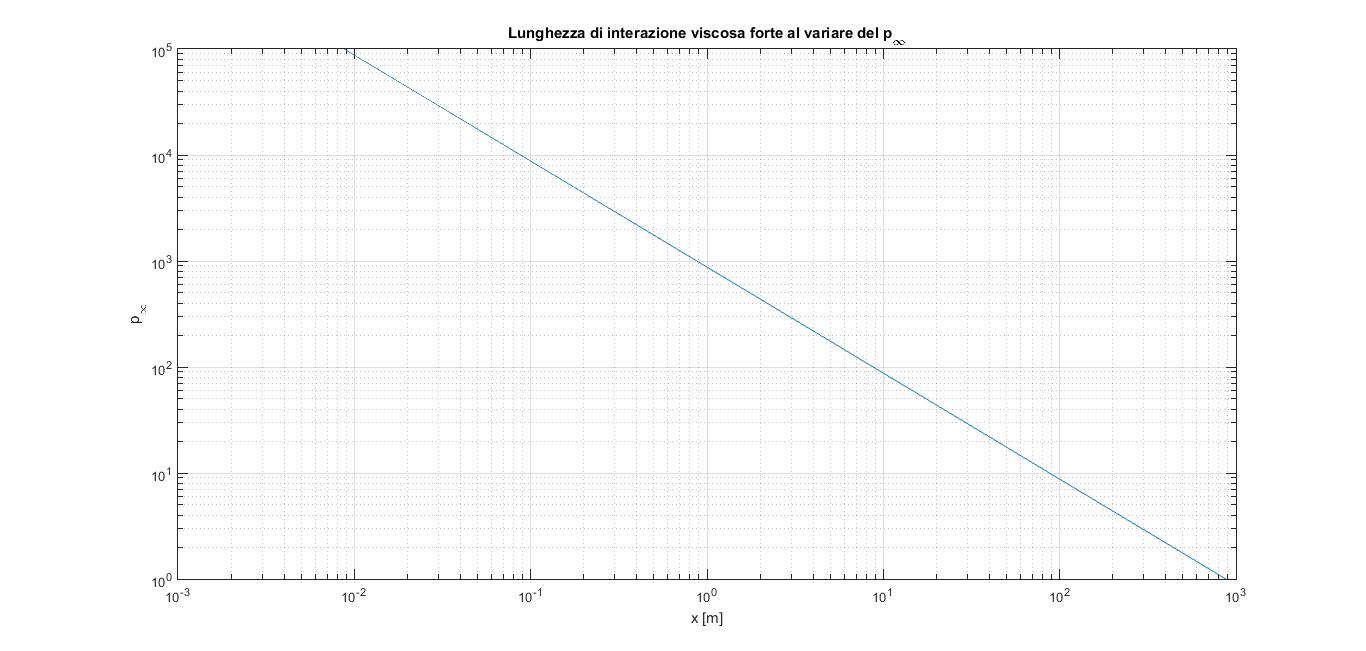
\includegraphics[width=150mm]{Immagini/L_p}
	\caption{Estensione della zona di interazione viscosa forte al variare della pressione}
\end{figure}
dato l'ordine delle grandezze in gioco, il grafico rapppresentato in figura � in scala logaritmica.\\
Si nota come la caratteristica $L=L(p_{\infty})$, avendo indicato con $L$ l'estensione della regione di interazione forte, sia di tipo lineare decrescente in scala logaritmica. Questo implica una riduzione della zona di interazione al diminuire della quota per un numero di Mach fissato abbastanza repentina.


\end{document}